\documentclass[11pt,a4paper]{article}
\usepackage[utf8]{inputenc}
\usepackage[vietnamese]{babel}
\usepackage{amsmath,amssymb}
\usepackage[version=4]{mhchem}
\usepackage{geometry}
\geometry{top=0.65cm,bottom=0.65cm,left=1.25cm,right=1.25cm,headheight=20pt,headsep=3pt,footskip=9pt}
\usepackage{graphicx}
\usepackage{xcolor}
\usepackage{tabularx}
\usepackage{array}
\usepackage{tikz}
\usepackage{multicol}
\usepackage{fancyhdr}
\usepackage{enumitem}

\definecolor{hfRed}{HTML}{D32F2F}
\definecolor{hfGreen}{HTML}{8BC390}
\definecolor{mainGreen}{HTML}{2E7D32}

\usepackage{ex_test}

\pagestyle{fancy}
\fancyhf{}
\renewcommand{\headrulewidth}{0.75pt}
\renewcommand{\headrule}{\hbox to\headwidth{\color{hfGreen}\leaders\hrule height \headrulewidth\hfill}}
\renewcommand{\footrulewidth}{0.75pt}
\renewcommand{\footrule}{\hbox to\headwidth{\color{hfGreen}\leaders\hrule height \footrulewidth\hfill}}

\fancyhead[L]{\small\itshape\color{hfRed}Tài liệu lưu hành nội bộ}
\fancyhead[R]{\small\color{hfRed}Thầy \textbf{TRẦN VĂN THẠNH} - 0777.470.803}

\fancyfoot[L]{\footnotesize\itshape\color{hfRed}CS1: 6/15 Nguyễn Hoàng, P. Kim Long, TP Huế \quad|\quad CS2: 24 Đặng Thái Thân, TP Huế}
\fancyfoot[R]{\small\textbf{\color{hfRed}Trang \thepage}}

\setlength{\parindent}{0pt}
\setlength{\parskip}{0.0pt}

\def\loigiai#1{}

\begin{document}
\Opensolutionfile{ans}[ans-de20-hs]

\noindent
\begin{minipage}[t]{0.48\textwidth}
	\textbf{SỞ GIÁO DỤC VÀ ĐÀO TẠO THỪA THIÊN HUẾ}\\
	\textbf{TRƯỜNG THPT HAI BÀ TRƯNG}\\
	\textbf{ĐỀ CHÍNH THỨC}\\
	\textit{(Đề thi có 04 trang)}
\end{minipage}\hfill
\begin{minipage}[t]{0.48\textwidth}
	\raggedleft
	\textbf{\color{mainGreen}ĐỀ KIỂM TRA ĐỊNH KỲ CHƯƠNG 7 (KIM LOẠI NHÓM IA \& IIA)}\\
	\textbf{MÔN: HOÁ HỌC -- LỚP 12}\\
	\textit{Thời gian làm bài: 50 phút (không kể thời gian phát đề)}\\
	\textbf{Mã đề thi: 120}
\end{minipage}


\vspace{1pt}
\noindent\textit{Họ, tên thí sinh: \dots\dots\dots\dots\dots\dots\dots\dots\dots\dots\dots\dots\dots\dots\dots\dots\dots\dots\dots\dots\dots\dots Lớp: \dots\dots\dots\dots SBD: \dots\dots\dots\dots}\\
\noindent\textit{(Cho biết nguyên tử khối: H = 1; C = 12; N = 14; O = 16; Na = 23; Mg = 24; Al = 27; P = 31; S = 32; Cl = 35,5; K = 39; Ca = 40; Fe = 56; Cu = 64; Zn = 65; Br = 80; Rb = 85,5; Ag = 108; Cs = 133; Ba = 137).}

\vspace{1pt}
\noindent
\textbf{PHẦN I (4,5 điểm -- 18 câu): Câu trắc nghiệm nhiều phương án lựa chọn.}\\
\textit{Thí sinh trả lời từ câu 1 đến câu 18. Mỗi câu hỏi thí sinh chỉ chọn một phương án.}

\begin{ex}
Sodium chloride là gia vị quan trọng trong thức ăn của con người. Công thức của sodium chloride là
\choice
{\ce{NaNO3}.}
{\ce{KNO3}.}
{\ce{NaCl}.}
{\ce{KCl}.}
\loigiai{}
\end{ex}

\begin{ex}
Tro thực vật được sử dụng như một loại phân bón cung cấp nguyên tố kali (potassium) cho cây trồng do chứa muối potassium carbonate. Công thức của potassium carbonate là
\choice
{\ce{KCl}.}
{\ce{KOH}.}
{\ce{NaCl}.}
{\ce{K2CO3}.}
\loigiai{}
\end{ex}

\begin{ex}
Khi nhiệt phân hoàn toàn \ce{NaHCO3} thì sản phẩm của phản ứng nhiệt phân là
\choice
{\ce{NaOH}, \ce{CO2}, \ce{H2}.}
{\ce{Na2O}, \ce{CO2}, \ce{H2O}.}
{\ce{Na2CO3}, \ce{CO2}, \ce{H2O}.}
{\ce{NaOH}, \ce{CO2}, \ce{H2O}.}
\loigiai{}
\end{ex}

\begin{ex}
Dãy gồm các kim loại đều phản ứng với nước ở nhiệt độ thường, tạo ra dung dịch có môi trường kiềm là
\choice
{Na, Ba, K.}
{Be, Na, Ca.}
{Na, Fe, K.}
{Na, Cr, K.}
\loigiai{}
\end{ex}

\begin{ex}
Cho phương trình hóa học của phản ứng nhiệt phân sau: $\ce{4M(NO3)_{$x$} ->[t^\circ] 2M2O_{$x$} + 4$x$NO2 + $x$O2}$. Kim loại M là
\choice
{Ca.}
{Mg.}
{K.}
{Ag.}
\loigiai{}
\end{ex}

\begin{ex}
Cho sơ đồ chuyển hoá hoá học sau:
\par\vspace{1pt}\centerline{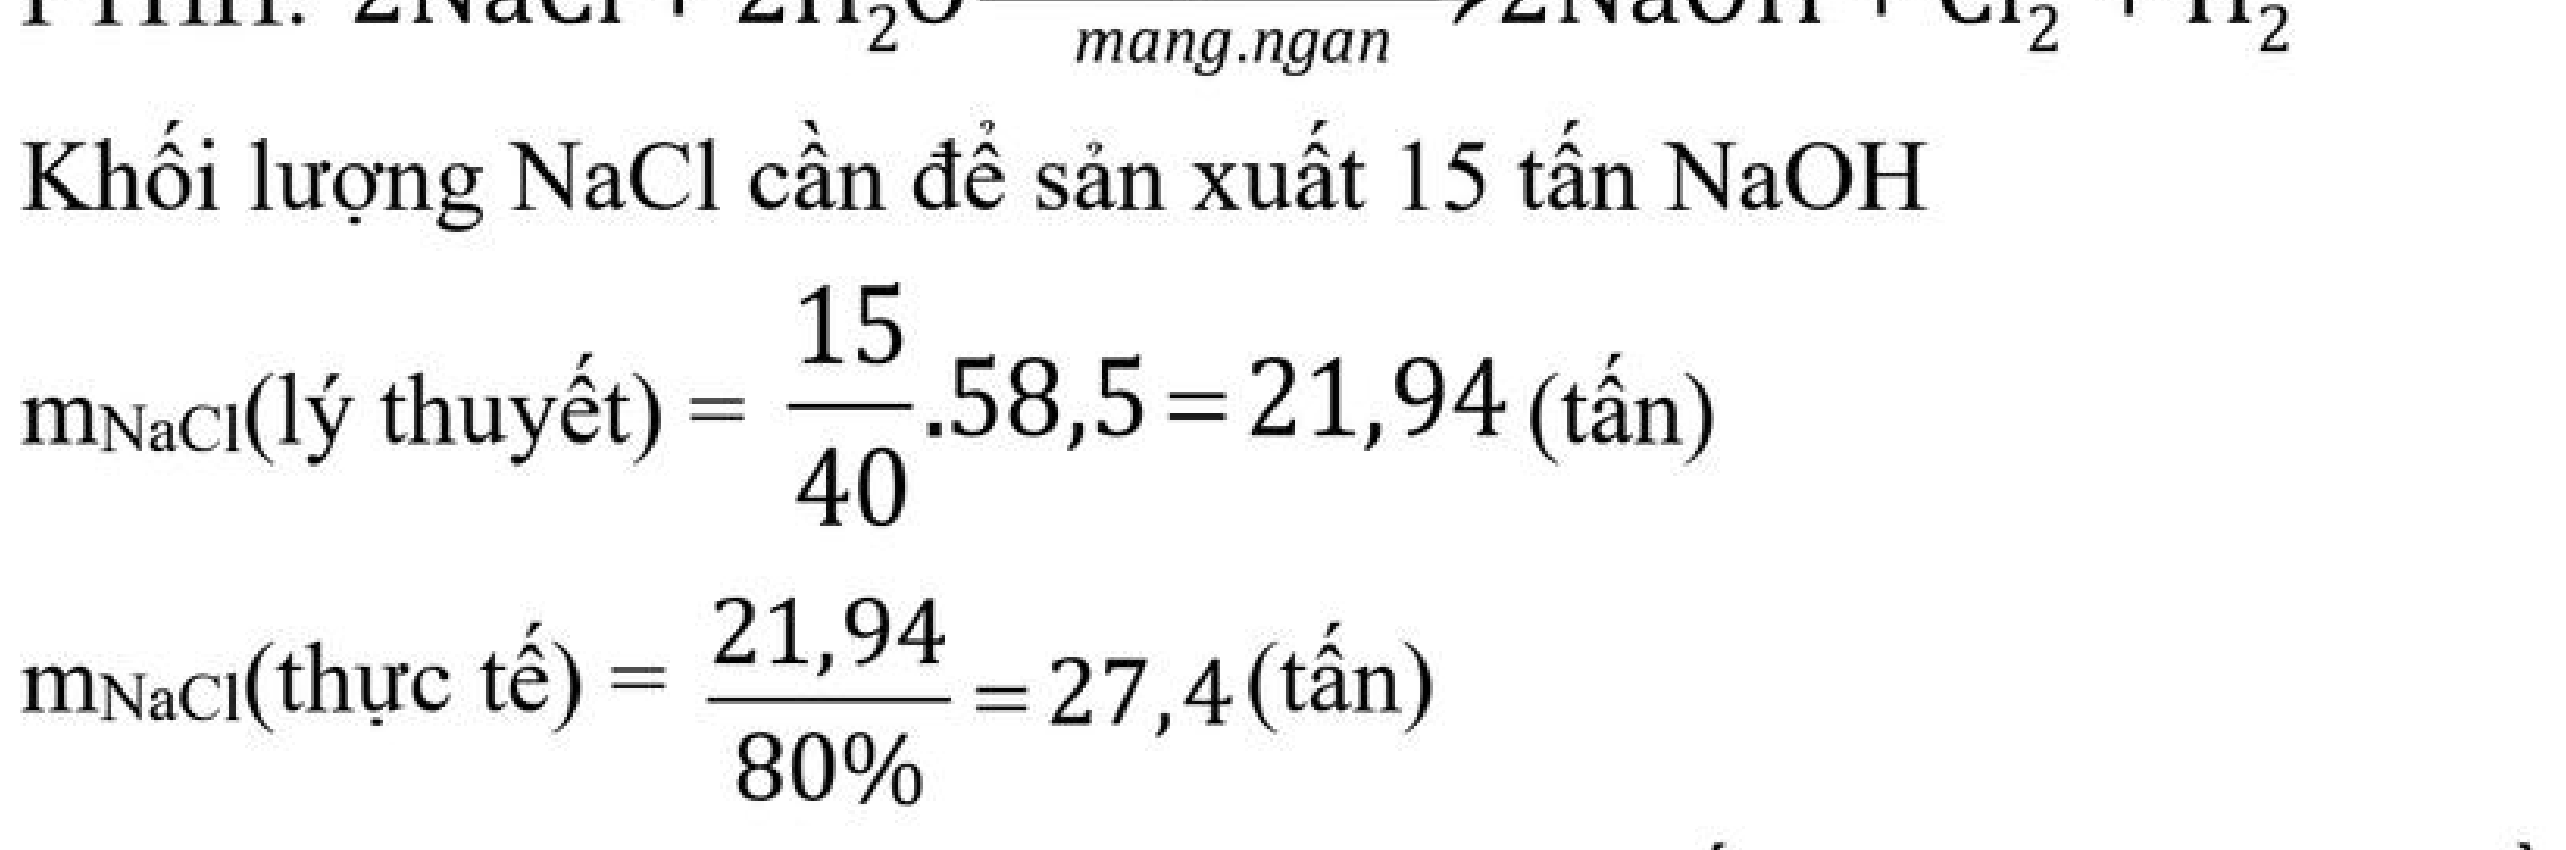
\includegraphics[height=1.45cm]{images_crop_de20/p1_cau6_so_do.png}}\vspace{1pt}
Chất X trong sơ đồ trên có thể là
\choice
{\ce{BaCO3}.}
{\ce{CaCO3}.}
{\ce{BaSO3}.}
{\ce{MgCO3}.}
\loigiai{}
\end{ex}

\begin{ex}
Phát biểu nào sau đây \textbf{không} đúng?
\choice
{Đun sôi nước cứng chỉ làm mềm nước cứng tạm thời.}
{Dung dịch \ce{Na2CO3} làm mềm nước cứng tạm thời, nước cứng vĩnh cửu.}
{Dung dịch \ce{NH4Cl} làm mềm nước cứng.}
{Cho dung dịch \ce{Ca(OH)2} vừa đủ làm mềm nước cứng tạm thời.}
\loigiai{}
\end{ex}

\begin{ex}
Để xử lí chất thải có tính acid trong công nghiệp và đời sống, người ta thường dùng
\choice
{nước vôi.}
{phèn chua.}
{giấm ăn.}
{muối ăn.}
\loigiai{}
\end{ex}

\begin{ex}
Hợp chất của calcium nào sau đây \textbf{không} gặp trong tự nhiên ở trạng thái tự do?
\choice
{\ce{CaCO3}.}
{\ce{CaSO4}.}
{\ce{Ca(HCO3)2}.}
{\ce{CaO}.}
\loigiai{}
\end{ex}

\newpage

\begin{ex}
Trong các kim loại sau, kim loại nào có tính khử mạnh nhất?
\choice
{K.}
{Al.}
{Mg.}
{Na.}
\loigiai{}
\end{ex}

\begin{ex}
Các dung dịch muối ăn, phèn chua, nước vôi trong được kí hiệu ngẫu nhiên là X, Y, Z. Một số kết quả thí nghiệm được ghi ở bảng sau:\\
-- Mẫu X + dung dịch phenolphthalein $\rightarrow$ Dung dịch chuyển sang màu hồng.\\
-- Mẫu Z + dung dịch \ce{BaCl2} $\rightarrow$ Xuất hiện kết tủa trắng.\\
Các dung dịch ban đầu (muối ăn, phèn chua, nước vôi trong) tương ứng lần lượt với các kí hiệu là
\choice
{Y, Z, X.}
{Z, X, Y.}
{X, Y, Z.}
{Y, X, Z.}
\loigiai{}
\end{ex}

\begin{ex}
Nguyên tố kim loại nhóm IIA được tìm thấy trong tự nhiên dưới dạng nào sau đây?\\
(1) Các cation $\ce{M^2+}$ trong nước sông, hồ, nước ngầm, nước biển.\\
(2) Các khoáng vật ít tan như carbonate, sulfate, silicate.\\
(3) Các hợp chất ít tan cấu tạo nên răng, xương động vật.
\choice
{(1) và (2).}
{(1) và (3).}
{(1), (2) và (3).}
{(2) và (3).}
\loigiai{}
\end{ex}

\begin{ex}
Barium phản ứng với nước dễ dàng hơn nhiều so với magnesium ở điều kiện thường là do các nguyên nhân nào sau đây?\\
(1) Barium có tính khử mạnh hơn magnesium.\\
(2) Độ tan của barium hydroxide trong nước cao hơn nhiều so với magnesium hydroxide.\\
(3) Bọt khí hydrogen sinh ra bám trên bề mặt magnesium nhiều hơn, cản trở phản ứng tiếp diễn.
\choice
{(1).}
{(1), (2) và (3).}
{(1) và (3).}
{(1) và (2).}
\loigiai{}
\end{ex}

\begin{ex}
Nhiệt độ phân huỷ thành oxide của các muối carbonate của kim loại nhóm IIA giảm dần theo dãy nào sau đây?
\choice
{\ce{MgCO3}, \ce{CaCO3}, \ce{SrCO3}, \ce{BaCO3}.}
{\ce{BaCO3}, \ce{SrCO3}, \ce{CaCO3}, \ce{MgCO3}.}
{\ce{BaCO3}, \ce{CaCO3}, \ce{SrCO3}, \ce{MgCO3}.}
{\ce{MgCO3}, \ce{BaCO3}, \ce{SrCO3}, \ce{CaCO3}.}
\loigiai{}
\end{ex}

\begin{ex}
Dãy các kim loại nào sau đây tác dụng nhanh với nước ở điều kiện thường?
\choice
{Be, Na, Ba.}
{Mg, Ca, Ba.}
{Li, Ca, Ba.}
{Sr, Sn, Ba.}
\loigiai{}
\end{ex}

\begin{ex}
Ion $\ce{Ca^2+}$ ($Z = 20$) đóng vai trò thiết yếu trong việc phát triển xương, giúp duy trì hoạt động của cơ bắp, kích thích máu lưu thông, điều tiết một số loại hormone,... Tổng số hạt proton và electron của ion $\ce{Ca^2+}$ là
\choice
{40.}
{42.}
{38.}
{18.}
\loigiai{}
\end{ex}

\begin{ex}
Đặc điểm nào sau đây là đặc điểm chung của nước có tính cứng vĩnh cửu và nước có tính cứng toàn phần?
\choice
{Đều có thể làm mềm bằng dung dịch \ce{Na3PO4}.}
{Đều không chứa anion \ce{HCO3-}.}
{Đều bị mất một phần tính cứng khi đun sôi nước.}
{Thành phần anion hoàn toàn giống nhau.}
\loigiai{}
\end{ex}

\begin{ex}
Cho các phát biểu sau:\\
(a) Tất cả các kim loại kiềm thổ đều tan trong nước ở nhiệt độ thường.\\
(b) Các kim loại kiềm có thể đẩy được kim loại yếu hơn ra khỏi dung dịch muối của chúng.\\
(c) Các ion $\ce{Na+}$, $\ce{Mg^2+}$, $\ce{Al^3+}$ có cùng cấu hình electron ở trạng thái cơ bản và đều có tính oxi hoá yếu.\\
(d) Các kim loại kiềm K, Rb, Cs tự bốc cháy khi tiếp xúc với nước.\\
(e) Kim loại magnesium có cấu trúc mạng tinh thể lục phương.\\
Trong các phát biểu trên, số phát biểu đúng là
\choice
{2.}
{3.}
{4.}
{5.}
\loigiai{}
\end{ex}

\newpage

\noindent
\textbf{PHẦN II (4,0 điểm -- 4 câu): Câu trắc nghiệm đúng sai.}\\
\textit{Thí sinh trả lời từ câu 1 đến câu 4. Trong mỗi ý a), b), c), d) ở mỗi câu, thí sinh chọn đúng hoặc sai.}

\setcounter{ex}{0}

\begin{ex}
Mỗi phát biểu sau đây về hợp chất của sodium là đúng hay sai?
\par\vspace{1pt}\centerline{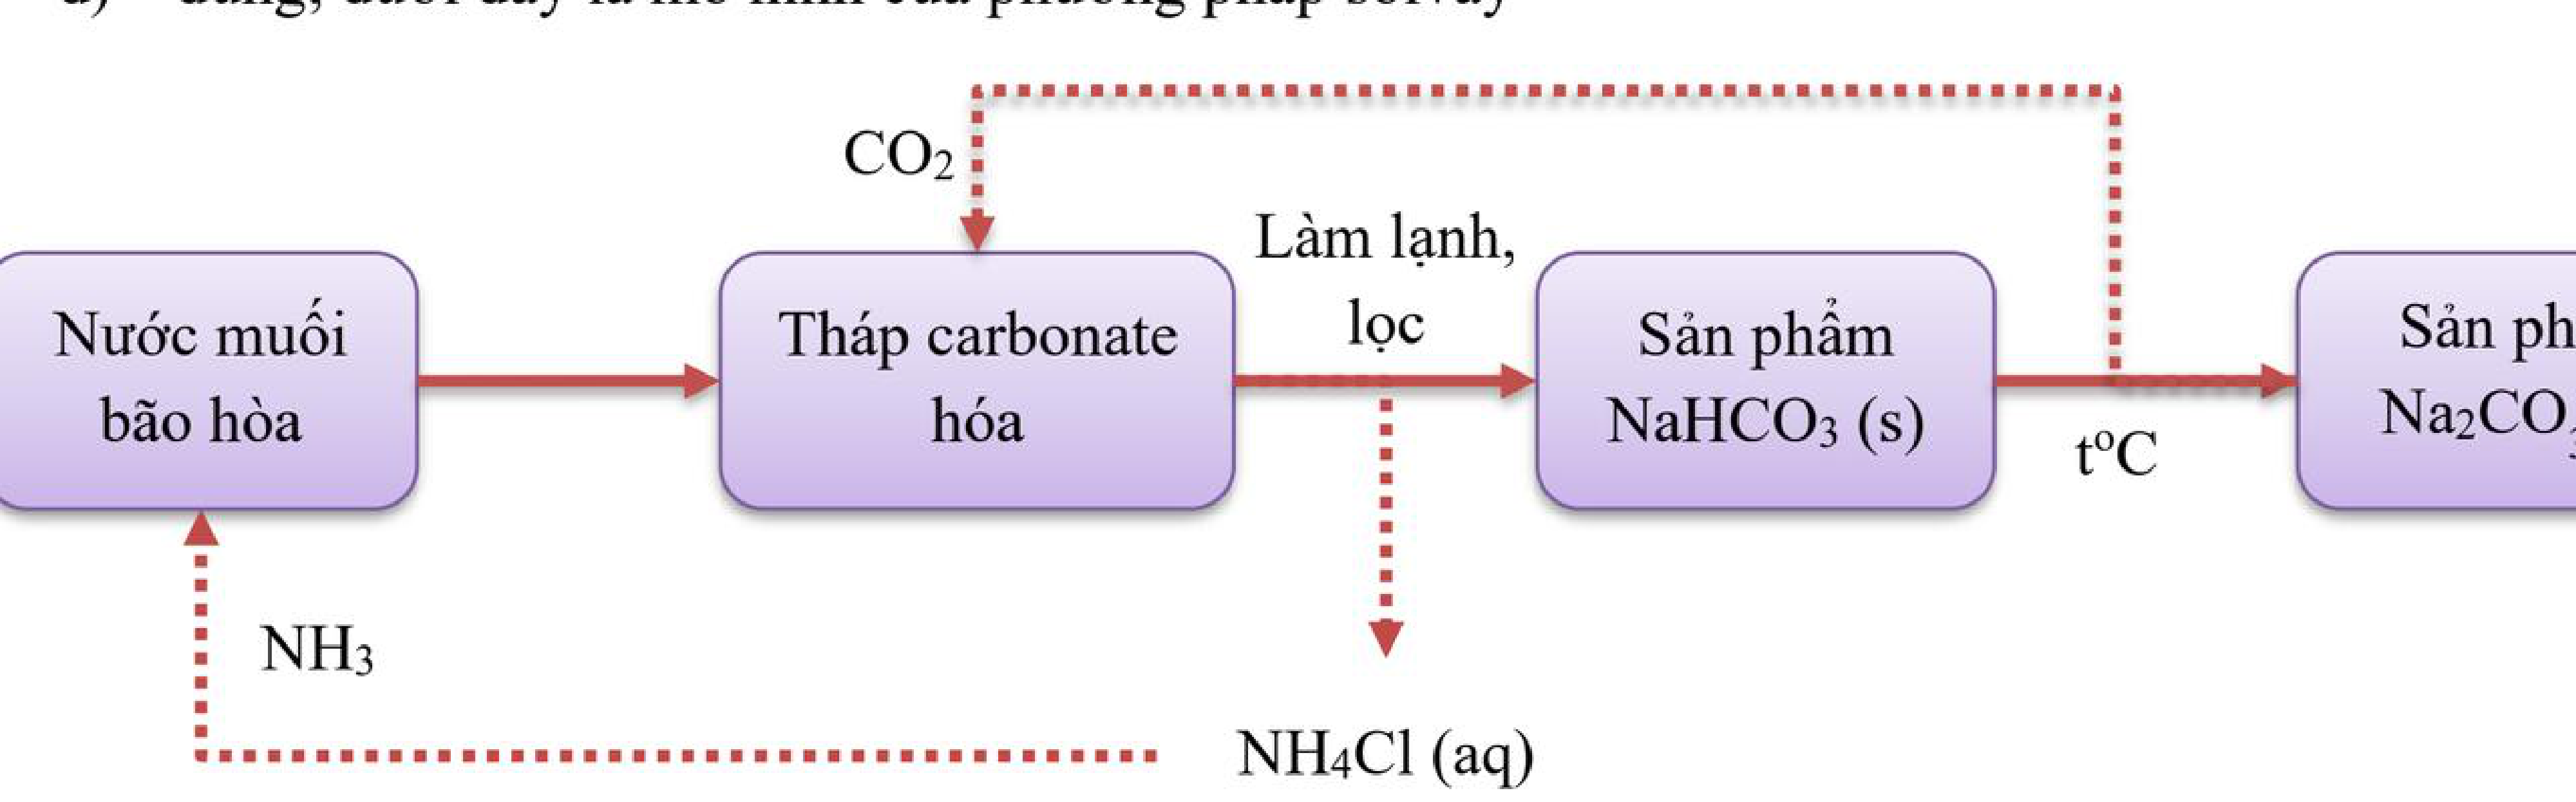
\includegraphics[height=2.3cm]{images_crop_de20/p2_cau1_solvay.png}}\vspace{1pt}
\choiceTF
{Điện phân dung dịch \ce{NaCl} có màng ngăn xốp thu được \ce{NaOH}, \ce{H2} và \ce{O2}.}
{\ce{NaHCO3} là hợp chất lưỡng tính.}
{\ce{Na2CO3} là nguyên liệu quan trọng để sản xuất thuỷ tinh.}
{Phương pháp Solvay sản xuất \ce{NaHCO3} từ nguyên liệu chính là \ce{NH3}, \ce{NaCl} và \ce{CO2}.}
\loigiai{}
\end{ex}

\begin{ex}
Sodium chloride là một hợp chất ion điển hình.
\choiceTF
{Ở trạng thái nóng chảy, sodium chloride có khả năng dẫn điện.}
{Sodium chloride có nhiệt độ nóng chảy cao.}
{Trong tinh thể sodium chloride ở điều kiện thường, các ion có thể di chuyển tự do.}
{Khi dùng búa đập vào hạt muối thì hạt muối bị biến dạng do có tính dẻo.}
\loigiai{}
\end{ex}

\begin{ex}
Mỗi phát biểu sau đây về kim loại kiềm thổ là đúng hay sai?
\choiceTF
{Các oxide của kim loại kiềm thổ đều bị khí CO khử thành kim loại tự do ở nhiệt độ cao.}
{Các kim loại Ca, Mg và Ba chỉ điều chế được bằng phương pháp điện phân nóng chảy.}
{Các kim loại Mg và Ba đều khử được ion \ce{Ag+} trong dung dịch thành Ag.}
{Cho kim loại Mg vào dung dịch \ce{FeCl3} dư thì không thu được kim loại Fe.}
\loigiai{}
\end{ex}

\begin{ex}
Hợp chất của kim loại kiềm có nhiều ứng dụng quan trọng trong thực tiễn.
\choiceTF
{Sodium carbonate khan (\ce{Na2CO3}, còn gọi là soda) được dùng trong công nghiệp thuỷ tinh, đồ gốm, bột giặt,...}
{Sodium hydrogencarbonate (\ce{NaHCO3}) được dùng trong công nghiệp thực phẩm làm bột nở và dùng làm thuốc giảm đau dạ dày.}
{Dung dịch \ce{NaCl} có nồng độ 0,9\% (nước muối sinh lý) được dùng để vệ sinh, súc miệng và sát khuẩn.}
{Chất thường được gọi là xút ăn da là KOH.}
\loigiai{}
\end{ex}

\newpage

\noindent
\textbf{PHẦN III (1,5 điểm -- 6 câu): Câu trắc nghiệm yêu cầu trả lời ngắn.}\\
\textit{Thí sinh trả lời từ câu 1 đến câu 6.}

\setcounter{ex}{0}

\begin{ex}
Cho các phát biểu sau:\\
(1) Nhúng đầu dây inox sạch vào dung dịch muối \ce{NaCl} rồi đưa vào ngọn lửa đèn khí thấy ngọn lửa nhuộm màu vàng tươi.\\
(2) Muối potassium carbonate tan tốt trong nước.\\
(3) Trong công nghiệp, một lượng lớn soda được dùng để sản xuất thuỷ tinh.\\
(4) Sodium hydrogencarbonate là chất rắn màu trắng, bền ở nhiệt độ thường.\\
(5) Điện phân dung dịch \ce{NaCl} có màng ngăn xốp thì ở cathode thu được kim loại Na.\\
Có bao nhiêu phát biểu đúng trong các phát biểu trên?
\par\noindent\textit{Trả lời:} \dotfill
\loigiai{}
\end{ex}

\begin{ex}
Baking soda bị phân huỷ khi đun nóng tạo thành soda, khí carbon dioxide và hơi nước. Tổng hệ số nguyên tối giản của các chất trong phương trình hoá học của phản ứng nhiệt phân baking soda là bao nhiêu?
\par\noindent\textit{Trả lời:} \dotfill
\loigiai{}
\end{ex}

\begin{ex}
Cho dãy các kim loại: Fe, Na, Ba, Ca. Có bao nhiêu kim loại trong dãy trên tác dụng được với nước ở nhiệt độ thường?
\par\noindent\textit{Trả lời:} \dotfill
\loigiai{}
\end{ex}

\begin{ex}
Có bao nhiêu chất bị phân huỷ bởi nhiệt độ trong dãy các chất sau: \ce{Na2CO3}, \ce{BaCO3}, \ce{CaSO4}, \ce{Ca(HCO3)2}, \ce{Mg(NO3)2}, \ce{NaHCO3}?
\par\noindent\textit{Trả lời:} \dotfill
\loigiai{}
\end{ex}

\begin{ex}
Ở điều kiện thường, kim loại calcium (Ca) kết tinh theo mạng tinh thể lập phương tâm diện với khối lượng riêng thực nghiệm $D = 1{,}55\text{ g/cm}^3$. Giả thiết các nguyên tử Ca là những hình cầu chiếm 74\% thể tích tinh thể, phần còn lại là các khe rỗng. Cho biết thể tích hình cầu $V = \frac{4}{3}\pi r^3$; số Avogadro $N_A = 6{,}023\times 10^{23}\text{ mol}^{-1}$; số $\pi = 3{,}1416$; khối lượng mol của Ca là $40\text{ g/mol}$. Tính bán kính nguyên tử Ca theo đơn vị picomet (pm) (làm tròn kết quả đến phần nguyên).
\par\noindent\textit{Trả lời:} \dotfill
\loigiai{}
\end{ex}

\begin{ex}
Khi điện phân 500 mL dung dịch \ce{NaCl} với điện cực trơ, có màng ngăn xốp đến khi khối lượng dung dịch giảm 5,475 gam thì ngừng điện phân, thu được dung dịch X (coi thể tích dung dịch thay đổi không đáng kể và nước bay hơi không đáng kể). Xác định giá trị pH của dung dịch X (làm tròn kết quả đến hai chữ số thập phân).
\par\noindent\textit{Trả lời:} \dotfill
\loigiai{}
\end{ex}

\Closesolutionfile{ans}
\end{document}
